% настройки в preamble.inc
\documentclass[14pt]{extarticle}

\usepackage[russian]{babel}
\usepackage[utf8]{inputenc}
\usepackage[T2A]{fontenc}

\usepackage{graphicx}  
\usepackage{amsfonts}
\usepackage{amsmath}
\usepackage{amssymb}
\usepackage{mathtools}
\usepackage{upgreek}
\usepackage{xfrac}


\usepackage{listings}

\lstset{
	captionpos=t,
	breaklines=true,         % автоматически переносить строки 
	breakatwhitespace=false, % переносить строки по пробелу
	%backgroundcolor=\color{mylightgray},rulecolor=\color{red},  % choose the background color; you must add \usepackage{color} or \usepackage{xcolor}; should come as last argument
	basicstyle=\footnotesize\ttfamily,        % the size of the fonts that are used for the code
	breakatwhitespace=false,         % sets if automatic breaks should only happen at whitespace
	breaklines=true,                 % sets automatic line breaking
	captionpos=t,                    % sets the caption-position to bottom
	commentstyle=\color{green},    % comment style
	extendedchars=false,              % lets you use non-ASCII characters; for 8-bits encodings only, does not work with UTF-8
	firstnumber=0,                % start line enumeration with line 1000
	frame=single,
	%rulesepcolor=\color{green},	                   % adds a frame around the code
	keepspaces=true,                 % keeps spaces in text, useful for keeping indentation of code (possibly needs columns=flexible)
	keywordstyle=\color{blue}\textbf,       % keyword style
	language=python,                 % the language of the code
	morekeywords={*,...},            % if you want to add more keywords to the set
	numbers=left,                    % where to put the line-numbers; possible values are (none, left, right)
	numbersep=5pt,                   % how far the line-numbers are from the code
	%numberstyle=\scriptsize\color{mygray}, % the style that is used for the line-numbers
	rulecolor=\color{black},         % if not set, the frame-color may be changed on line-breaks within not-black text (e.g. comments (green here))
	showspaces=false,                % show spaces everywhere adding particular underscores; it overrides 'showstringspaces'
	showstringspaces=false,          % underline spaces within strings only
	showtabs=false,                  % show tabs within strings adding particular underscores
	stepnumber=1,                    % the step between two line-numbers. If it's 1, each line will be numbered
	%stringstyle=\color{mymauve},     % string literal style
	tabsize=4,	                   % sets default tabsize to 2 spaces
	%title=\lstname                   % show the filename of files included with \lstinputlisting; also try caption instead of title
}

\lstset{
	captionpos=t,
	breaklines=true,         % автоматически переносить строки 
	breakatwhitespace=false, % переносить строки по пробелу
	%backgroundcolor=\color{mylightgray},rulecolor=\color{red},  % choose the background color; you must add \usepackage{color} or \usepackage{xcolor}; should come as last argument
	basicstyle=\footnotesize\ttfamily,        % the size of the fonts that are used for the code
	breakatwhitespace=false,         % sets if automatic breaks should only happen at whitespace
	breaklines=true,                 % sets automatic line breaking
	captionpos=t,                    % sets the caption-position to bottom
	commentstyle=\color{green},    % comment style
	extendedchars=false,              % lets you use non-ASCII characters; for 8-bits encodings only, does not work with UTF-8
	firstnumber=0,                % start line enumeration with line 1000
	frame=single,
	%rulesepcolor=\color{green},	                   % adds a frame around the code
	keepspaces=true,                 % keeps spaces in text, useful for keeping indentation of code (possibly needs columns=flexible)
	keywordstyle=\color{blue}\textbf,       % keyword style
	language=SQL,                 % the language of the code
	morekeywords={*,...},            % if you want to add more keywords to the set
	numbers=left,                    % where to put the line-numbers; possible values are (none, left, right)
	numbersep=5pt,                   % how far the line-numbers are from the code
	%numberstyle=\scriptsize\color{mygray}, % the style that is used for the line-numbers
	rulecolor=\color{black},         % if not set, the frame-color may be changed on line-breaks within not-black text (e.g. comments (green here))
	showspaces=false,                % show spaces everywhere adding particular underscores; it overrides 'showstringspaces'
	showstringspaces=false,          % underline spaces within strings only
	showtabs=false,                  % show tabs within strings adding particular underscores
	stepnumber=1,                    % the step between two line-numbers. If it's 1, each line will be numbered
	%stringstyle=\color{mymauve},     % string literal style
	tabsize=4,	                   % sets default tabsize to 2 spaces
	%title=\lstname                   % show the filename of files included with \lstinputlisting; also try caption instead of title
}

\usepackage{enumerate}
%\usepackage{multirow}
%\usepackage{tikz}
%\usetikzlibrary{arrows,positioning,shadows}
%\usepackage{paralist,array}

\usepackage{geometry}
\geometry{right=20mm}
\geometry{left=30mm}
\geometry{bottom=20mm}
\geometry{ignorefoot}% считать от нижней границы текста

\setlength{\parindent}{1.25 cm}
\setlength{\parskip}{1ex}
\renewcommand{\baselinestretch}{1.5}

\usepackage[toc,page]{appendix}

\usepackage{titlesec}
\titleformat{\section}
  {\normalfont\fontsize{14}{14}\bfseries}{\thesection}{1em}{}
\titleformat{\subsection}
  {\normalfont\fontsize{14}{14}\bfseries}{\thesubsection}{1em}{}

\usepackage[intoc]{nomencl}
\renewcommand{\nomname}{Обозначения и сокращения}
\makenomenclature

%Подписи
\usepackage		[margin		= 10	pt,
%					font		= footnotesize, 
					labelfont	= bf, 
					labelsep	= endash, 
					labelfont	= bf,
%					textfont	= sl,
					margin		= 0 	pt,  
					aboveskip 	= 4		pt, 
					belowskip 	= -6	pt,
					figurename= Рисунок] {caption}
\usepackage		[margin		= 10	pt,
					font		= footnotesize, 
					labelfont	= bf, 
					labelsep	= endash, 
					labelfont	= bf,
					textfont	= sl,
					margin		= 0 	pt,  
					aboveskip 	= 4		pt, 
					belowskip 	= 6	pt]	{subcaption}


\newcommand\Referat{%реферат
	\chapter*{Реферат}%
}

\addto\captionsrussian{%
	\def\contentsname{%
		Содержание}%
	\def\bibname{%
		Список~
		использованных~
		источников}%
}


\usepackage{enumitem}
\usepackage{kosrem}
\usepackage{gensymb}


\begin{document}




\setcounter{page}{3}

% СОДЕРЖАНИЕ 
\clearpage
\tableofcontents

% ВВЕДЕНИЕ
\clearpage
\section*{Введение}
\addcontentsline{toc}{section}{Введение}
В современном мире каждая сфера деятельности связана с использованием информационных технологий, в частности, сети Интернет. Сейчас уже невозможно представить какую-либо компанию или организацию без своего сайта.

Целью данной работы является разработка базы данных и приложения для библиотеки. 

Для достижения поставленной цели необходимо решить следующие задачи:
\begin{itemize}
	\item[1)] формализовать задание, выделив соответствующих акторов и их функционал;
	\item[2)] провести анализ СУБД и выбрать наиболее подходящую;
	\item[3)] спроектировать базу данных;
	\item[4)] спроектировать архитектуру приложения;
	\item[5)] разработать приложение.
\end{itemize}

% АНАЛИТИЧЕСКАЯ ЧАСТЬ
\clearpage
\section{Аналитический раздел}
В данном разделе будет поставлена задача, рассмотрены возможные пользователи системы, модели данных и СУБД.

\subsection{Постановка задачи}
Необходимо разработать программу, предоставляющую интерфейс для получения информации о книгах и совершения действий с ними, доступных в зависимости от роли пользователя.
\subsection{Пользователи системы}
\subsubsection{Гость}
Гость — это неавторизованный пользователь. Он может только просматривать список книг и авторов и информацию о них.
\subsubsection{Читатель}
Читатель - это авторизированный пользователь. Он может подать заявку на взятие книги, если она у него не на руках, и на её сдачу в противном случае. Также ему доступны списки книг, на которые он оставил заявки, которые у него на руках и которые он уже прочел и сдал.
\subsubsection{Библиотекарь} 
Библиотекарь - это авторизованный пользователь, контролирующий выдачу книг. Он одобряет заявки читателей, и добавляет новые книги и авторов в БД.
\subsubsection{Администратор}
Администратор является авторизированным пользователем с повышенным уровнем полномочий — он может регистрировать новых пользователей и удалять существующих.
\subsection{Анализ моделей баз данных}
Модель базы данных - это тип модели данных, которая определяет логическую структуру базы данных и в корне определяет, каким образом данные могут храниться, организовываться и обрабатываться.

\subsubsection{Иерархическая база данных}
Иерархическая модель базы данных подразумевает, что элементы организованы в структуры, связанные между собой иерархическими или древовидными связями. Родительский элемент может иметь несколько дочерних элементов. Но у дочернего элемента может быть только один предок.

Иерархические базы данных графически могут быть представлены как перевернутое дерево, состоящее из объектов различных уровней. Верхний уровень (корень дерева) занимает один объект, второй - объекты второго уровня и так далее. 

Такая модель подразумевает возможность существования одинаковых (преимущественно дочерних) элементов. Данные здесь хранятся в серии записей с прикреплёнными к ним полями значений. Модель собирает вместе все экземпляры определённой записи в виде «типов записей» — они эквивалентны таблицам в реляционной модели, а отдельные записи — столбцам таблицы.

\subsubsection{Сетевая модель базы данных}
Сетевая модель базы данных подразумевает, что у родительского элемента может быть несколько потомков, а у дочернего элемента — несколько предков. Записи в такой модели связаны списками с указателями. 

Сетевая модель состоит из множества записей, которые могут быть владельцами или членами групповых отношений. Связь между записью-владельцем и записью-членом также имеет вид 1:N.

Сетевая модель позволяет иметь несколько предков и потомков, формирующих решётчатую структуру.

На рисунке \ref{img:set} представлен пример сетевой модели базы данных.

\begin{figure}[h!]
	\centering
	\includegraphics[scale=1]{img/"Иерархическая модель базы данных.png"}
	\caption{Иерархическая модель базы данных}
	\label{img:set}
\end{figure}

\subsubsection{Реляционная модель базы данных}
В реляционной модели, в отличие от иерархической или сетевой, не существует физических отношений. Вся информация хранится в виде таблиц (отношений), состоящих из рядов и столбцов. А данные двух таблиц связаны общими столбцами, а не физическими ссылками или указателями. Для манипуляций с рядами данных существуют специальные операторы.

Реляционные таблицы обладают следующими свойствами:
\begin{itemize}
	\item[1)] все значения атомарны;
	\item[2)] каждый ряд уникален;
	\item[3)] порядок столбцов не важен;
	\item[4)] порядок рядов не важен;
	\item[5)] у каждого столбца есть своё уникальное имя.
\end{itemize}

Термин «реляционный» означает, что теория основана на математическом понятии отношение (relation). В качестве неформального синонима термину «отношение» часто встречается слово таблица. Необходимо помнить, что «таблица» есть понятие нестрогое и неформальное и часто означает не «отношение» как абстрактное понятие, а визуальное представление отношения на бумаге или экране. Некорректное и нестрогое использование термина «таблица» вместо термина «отношение» нередко приводит к недопониманию.

\subsubsection{Выбор модели данных}
В качестве модели данных была выбрана реляционная модель, так как структура данных однозначно определена, структура данных не является быстроизменяющейся и данные подчиняются строгим правилам и ограничениям.

\subsection{Вывод}
В данном разделе была поставлена задача, рассмотрены возможные пользователи системы, проанализированы модели данных и СУБД.


%КОНСТРУКТОРСКИЙ РАЗДЕЛ
\clearpage
\section{Конструкторский раздел}
В данном разделе будут рассмотрены сценарии пользователей, спроектирована база данных, описана ролевая модель и разработанны триггеры.
\subsection{Сценарии пользователей}
Необходимо определить функционал каждого из пользователей. 
\subsubsection{Гость}
Гость - это неавторизованный пользователь, у которого есть только одна возможность - авторизоваться. На рисунке \ref{img:UseCaseGuest} представлена Use-Case-диаграмма для гостя.

\begin{figure}[h!]
	\centering
	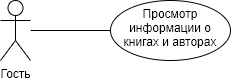
\includegraphics[scale=1]{img/UseCaseGuest.png}
	\caption{Сценарии для гостя.}
	\label{img:UseCaseGuest}
\end{figure}
\clearpage

\subsubsection{Любой авторизированный пользователь}
Функционал, предоставляемый каждому авторизированному пользователю (читателю, библиотекарю, администратору):
\begin{itemize}
	\item[1)] просмотр списка книг;
	\item[2)] просмотр информации о книге;
	\item[3)] просмотр списка авторов;
	\item[4)] просмотр информации о книге.      
\end{itemize}
\subsubsection{Читатель}
Дополнительная функциональность, предоставляемая пользователю читатель:
\begin{itemize}
	\item[1)] оставить заявку на получение книги;
	\item[2)] оставить заявку на сдачу книги;
	\item[3)] просмотр списка всех заявок;
	\item[4)] просмотр списка всех книг на руках;
	\item[5)] просмотр списка всех прочитанных и сданных книг.
\end{itemize}
На рисунке \ref{img:UseCaseReader} представлена Use-Case-диаграмма для читателя.
\begin{figure}[h!]
	\centering
	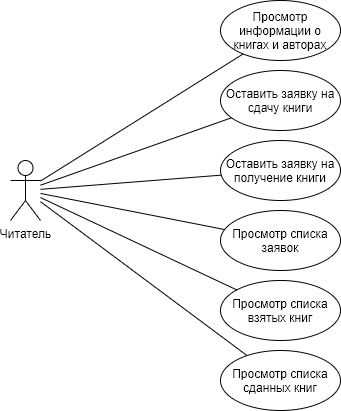
\includegraphics[scale=1]{img/UseCaseReader.png}
	\caption{Сценарии для читателя.}
	\label{img:UseCaseReader}
\end{figure}
\clearpage

\subsubsection{Библиотекарь}
Дополнительная функциональность, предоставляемая пользователю библиотекарь:
\begin{itemize}
	\item[1)] просмотр и одобрение всех заявок на выдачу книг;
	\item[2)] просмотр и одобрение всех заявок на сдачу книг; 
	\item[3)] добавление нового автора;
	\item[4)] добавление новой книги существующему автору.    
\end{itemize}
На рисунке \ref{img:UseCaseLibrarian} представлена Use-Case-диаграмма для библиотекаря.
\begin{figure}[h!]
	\centering
	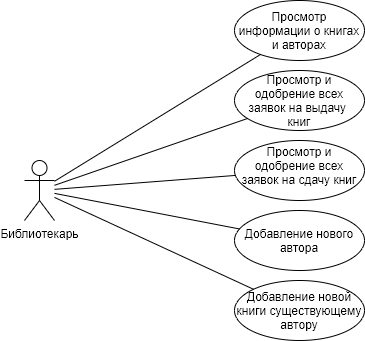
\includegraphics[scale=1]{img/UseCaseLibrarian.png}
	\caption{Сценарии для библиотекаря.}
	\label{img:UseCaseLibrarian}
\end{figure}
\clearpage

\subsubsection{Администратор}
Дополнительная функциональность, предоставляемая пользователю администратор:
\begin{itemize}
	\item[1)] зарегистрировать нового пользователя;
	\item[2)] удалить пользователя.  
\end{itemize}
На рисунке \ref{img:UseCaseAdmin} представлена Use-Case-диаграмма для администратора.
\begin{figure}[h!]
	\centering
	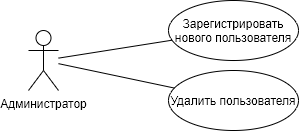
\includegraphics[scale=1]{img/UseCaseAdmin.png}
	\caption{Сценарии для администратора.}
	\label{img:UseCaseAdmin}
\end{figure}
\newpage

\subsection{Проектирование базы данных}
\subsubsection{Формализация сущностей системы}
Необходимо выделить сущности предметной области и построить ER-диаграмму. 
На рисунке \ref{img:ER} представлена ER-диаграмма системы.
\begin{figure}[h!]
	\centering
	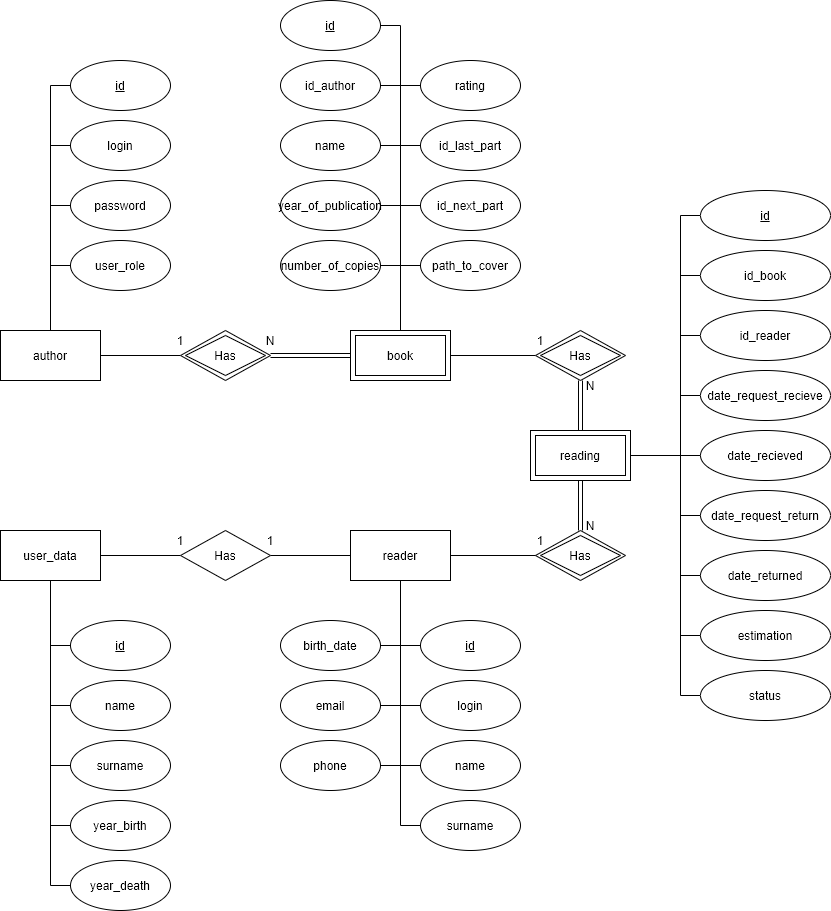
\includegraphics[scale=0.5]{img/ER.png}
	\caption{ER-диаграмма системы.}
	\label{img:ER}
\end{figure}
\newpage
Выделенные сущности:
\begin{itemize}
	\item[1)] author - таблица, в которой хранится информация об авторах;
	\item[2)] book - таблица, в которой хранится информация об книгах;
	\item[3)] user\_data - таблица, в которой хранятся данные для авторизации зарегистрированных пользователей;
	\item[4)] reader - таблица, в которой хранится информация о читателях;
	\item[5)] reading - таблица, в которой хранится информация о взятых книгах.
\end{itemize}

Атрибут status таблицы reading может принимать 4 значения:
\begin{itemize}
	\item[1)] 'request\_recieve' - подана заявка на взятие книги;
	\item[2)] 'in\_reading' - книга выдана;
	\item[3)] 'request\_return' - подана заявка на сдачу книги;
	\item[4)] 'returned' - книга сдана.
\end{itemize}

\subsubsection{Ролевая модель}
На уровне базы данных выделена следующая ролевая модель:
\begin{itemize}
	\item[1)] guest - гость;
	\item[2)] reader - читатель;
	\item[3)] librarian - библиотекарь;
	\item[4)] admin - администратор.  
\end{itemize}
Использование ролевой модели на уровне базы данных гарантирует безопасность доступа к объектам базы данных.

\textbf{Гость}\\
Пользователь с ролью guest имеет следующие права:
\begin{itemize}
	\item[1)] SELECT над таблицей author;
	\item[2)] SELECT над таблицей book; 
	\item[3)] SELECT над таблицей user\_data.    
\end{itemize}

\textbf{Читатель}\\
Пользователь с ролью reader имеет следующие права:
\begin{itemize}
	\item[1)] SELECT над таблицей book;
	\item[2)] SELECT, INSERT, UPDATE над таблицей reading; 
	\item[3)] SELECT над таблицей author;
	\item[4)] SELECT над таблицей reader;
	\item[5)] SELECT над таблицей user\_data.
\end{itemize}

\textbf{Библиотекарь}\\
Пользователь с ролью librarian имеет следующие права:
\begin{itemize}
	\item[1)] SELECT, INSERT, DELETE, UPDATE над таблицей book;
	\item[2)] SELECT, INSERT, DELETE, UPDATE над таблицей reading; 
	\item[3)] SELECT, INSERT, DELETE, UPDATE над таблицей author;
	\item[4)] SELECT над таблицей reader;
	\item[5)] SELECT над таблицей user\_data.
\end{itemize}

\textbf{Администратор}\\
Пользователь с ролью admin обладает всеми правами.

\subsubsection{Триггеры}
Для обеспечения целостности данных необходимо добавить соответствующие триггеры. 

При возврате книги, в соответствующей записи в таблице reading полю status присваивается значение 'returned'. Также при возврате книги ей может быть дана оценка - estimation. На основании всех данных оценок строится рейтинг книги. На рисунке \ref{img:update_rating_trigger} представлен алгоритм триггера, обеспечивающего актуальность рейтинга.

\begin{figure}[h!]
	\centering
	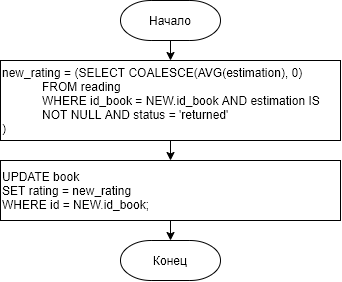
\includegraphics[scale=1]{img/update_rating_trigger.png}
	\caption{Алгоритм триггера рейтинга.}
	\label{img:update_rating_trigger}
\end{figure}
\newpage

При выдаче или сдаче книги, в соответствующей записи в таблице reading полю status присваивается значение 'in\_reading' или 'returned' соответственно. Триггер должен изменять значение number\_of\_copies соответствующей книги - количество оставшихся экземпляров книги. На рисунке \ref{img:update_number_of_copies_trigger} представлен алгоритм триггера, обеспечивающего актуальность количества оставшихся экземпляров книги.

\begin{figure}[h!]
	\centering
	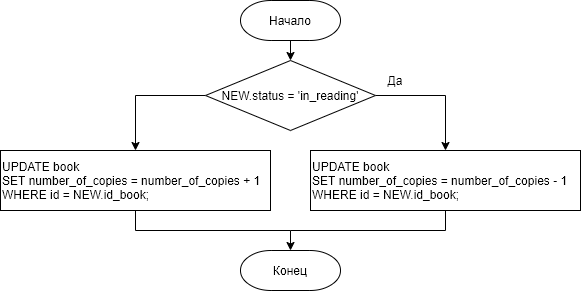
\includegraphics[scale=0.85]{img/update_number_of_copies_trigger.png}
	\caption{Алгоритм триггера рейтинга.}
	\label{img:update_number_of_copies_trigger}
\end{figure}
\newpage

При добавлении новой книги нужно проконтролировать, что её ссылки на предыдущую и следующую части однозначны. На рисунке \ref{img:parts_connect_trigger} представлен алгоритм триггера, обеспечивающего целостность связи частей серии.

\begin{figure}[h!]
	\centering
	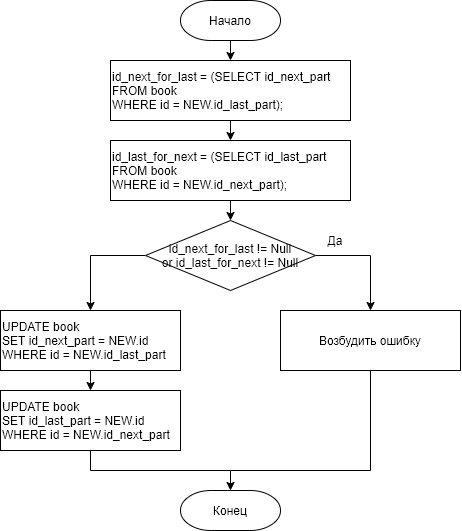
\includegraphics[scale=0.9]{img/parts_connect_trigger.png}
	\caption{Алгоритм триггера целостности частей серии.}
	\label{img:parts_connect_trigger}
\end{figure}
\newpage

\subsection{Вывод}
В данном разделе были рассмотрены сценарии пользователей, спроектирована база данных, описана ролевая модель и приведены схемы алгоритмов разработанных триггеров.

\newpage
%ТЕХНОЛОГИЧЕСКИЙ РАЗДЕЛ
\section{Технологический раздел}
В данном разделе будут выбраны средства реализации поставленной задачи, создана база данных и ролевая модель, разработано приложение.
\subsection{Анализ СУБД}
СУБД — комплекс программ, позволяющих создать базу данных (БД) и манипулировать данными (вставлять, обновлять, удалять и выбирать). Система обеспечивает безопасность, надёжность хранения и целостность данных, а также предоставляет средства для администрирования БД. Самыми популярными СУБД являются MySQL, Microsoft SQL Server, PostgreSQL и Oracle.
\subsubsection{MySQL}
MySQL — реляционная СУБД с открытым исходным кодом, главными плюсами которой являются ее скорость и гибкость, которая обеспечена поддержкой большого количества различных типов таблиц.

Кроме того, это надежная бесплатная система с простым интерфейсом и возможностью синхронизации с другими базами данных. В совокупности эти факторы позволяют использовать MySQL как крупным корпорациям, так и небольшим компаниям.

Преимущества:
\begin{itemize}
	\item[1)] простота в использовании;
	\item[2)] обширный функционал;
	\item[3)] безопасность;
	\item[4)] масштабируемость;
	\item[5)] скорость.    
\end{itemize}
Недостатки: недостаточная надежность;
\subsubsection{Microsoft SQL Server}
Система позволяет синхронизироваться с другими программными продуктами компании Microsoft, а также обеспечивает надежную защиту данных и простой интерфейс, однако отличается высокой стоимостью лицензии и повышенным потреблением ресурсов.

Преимущества:
\begin{itemize}
	\item[1)] СУБД масштабируется;
	\item[2)] простота в использовании;
	\item[3)] возможность интеграции с другими продуктами Microsoft.  
\end{itemize}
Недостатки:
\begin{itemize}
	\item[1)] высокая стоимость продукта для юридических лиц; 
	\item[2)] возможны проблемы в работе служб интеграции импорта файлов;
	\item[3)] высокая ресурсоемкость SQL Server.  
\end{itemize}
\subsubsection{PostgreSQL}
PostgreSQL — это популярная свободная объектно-реляционная система управления базами данных. PostgreSQL базируется на языке SQL и поддерживает многочисленные возможности.

Преимущества:
\begin{itemize}
	\item[1)] бесплатное ПО с открытым исходным кодом;
	\item[2)] большое количество дополнений;
	\item[3)] расширения;   
\end{itemize}
Недостатки:
\begin{itemize}
	\item[1)] производительность;
	\item[2)] популярность;  
\end{itemize}
\subsubsection{Oracle}
Oracle – это объектно-реляционная система управления базами данных.

Преимущества:
\begin{itemize}
	\item[1)] поддержка огромных баз данных;
	\item[2)] быстрая обработка транзакций;
	\item[3)] большой и постоянно развивающийся функционал.   
\end{itemize}
Недостатки:
\begin{itemize}
	\item[1)] высокая стоимость; 
	\item[2)] значительные вычислительные ресурсы. 
\end{itemize}

\begin{figure}[h!]
	\centering
	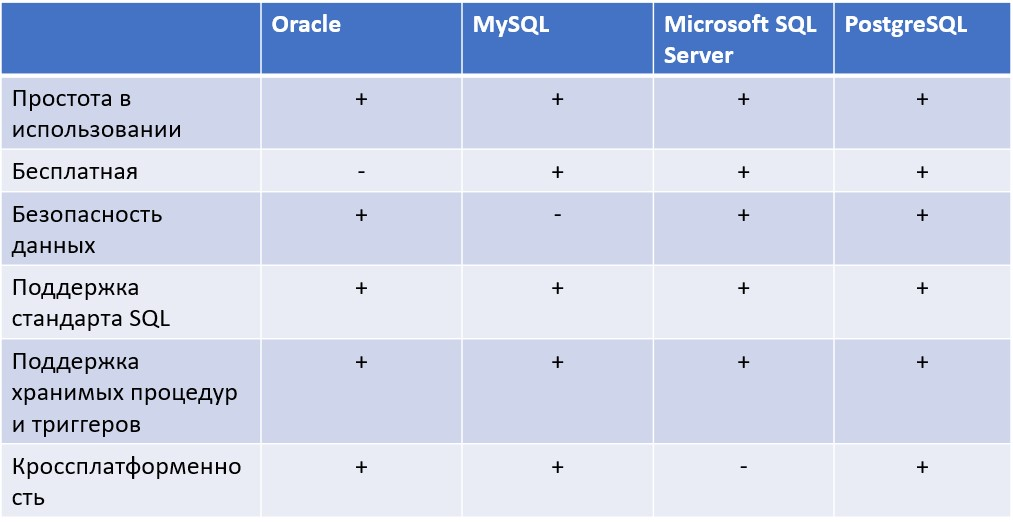
\includegraphics[scale=0.6]{img/subd.jpg}
	\caption{Анализ СУБД.}
	\label{img:subd}
\end{figure}

\subsection{Средства реализации поставленной задачи}
Для разработки программы выбран язык Python по причине совмещения нескольких парадигм программирования, а также из-за большого разнообразия представленных библиотек и фреймворков для создания веб-приложения.

В качестве среды разработки был выбран PyCharm, так как с его помощью удобно работать и с python-файлами, и html-страницами. Среда обладает кроссплатформенностью и большим выбором настроек проекта.

Для создания данного проекта в качестве инструмента, который облегчит процесс создания веб-приложения, был выбран фреймворк Flask. Благодаря его простоте и гибкости, разработчик может сам выбрать способ реализации тех или иных задач.

Для данной задачи PostgreSQL\cite{psql} выигрывает по многим параметрам и поэтому было решено использовать именно эту СУБД.

\subsection{Создание базы данных}
Необходимо построить диаграмму БД по выделенным сущностям. На рисунке \ref{img:DB} представлена диаграмма БД.
\begin{figure}[h!]
	\centering
	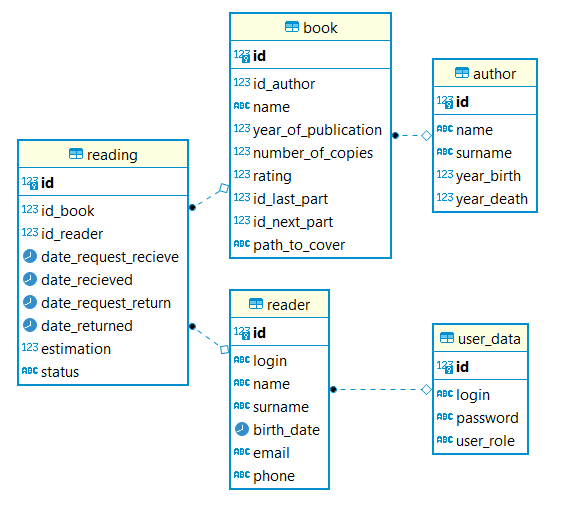
\includegraphics[scale=1]{img/DB.png}
	\caption{Диаграмма БД.}
	\label{img:DB}
\end{figure}
\newpage
\subsection{Создание таблиц}
Далее представлены листинги создания таблиц с указанием типов данных каждого столбца.

\textbf{Таблица user\_data.}
\begin{lstlisting}[label={lst:user_data},caption=Создание таблицы user\_data., language=SQL]
CREATE type user_role_t as enum (
	'admin',
	'librarian',
	'reader'
);

CREATE TABLE user_data (
	id SERIAL NOT NULL PRIMARY KEY,
	login TEXT NOT NULL UNIQUE, 
	password TEXT NOT NULL, 
	user_role user_role_t NOT NULL
);
\end{lstlisting}

\textbf{Таблица reader.}
\begin{lstlisting}[label={lst:reader},caption=Создание таблицы reader., language=SQL]
CREATE TABLE IF NOT EXISTS reader (
	id SERIAL NOT NULL PRIMARY KEY,
	login TEXT REFERENCES user_data(login) ON DELETE CASCADE NOT NULL,
	name TEXT NOT NULL,
	surname TEXT NOT NULL,
	birth_date DATE NOT NULL,
	email TEXT NOT NULL UNIQUE CHECK(email SIMILAR TO '%@%.%'),
	phone TEXT NOT NULL UNIQUE CHECK(phone SIMILAR TO '[0-9]{11}')
);
\end{lstlisting}

\textbf{Таблица author.}
\begin{lstlisting}[label={lst:author},caption=Создание таблицы author., language=SQL]
CREATE TABLE IF NOT EXISTS author (
	id SERIAL NOT NULL PRIMARY KEY,
	name TEXT NOT NULL,
	surname TEXT NOT NULL,
	year_birth INT NOT NULL,
	year_death INT
);
\end{lstlisting}

\textbf{Таблица book}.
\begin{lstlisting}[label={lst:book},caption=Создание таблицы book., language=SQL]
CREATE TABLE IF NOT EXISTS book (
	id SERIAL NOT NULL PRIMARY KEY,
	id_author INT REFERENCES author(id) ON DELETE CASCADE NOT NULL,
	name TEXT UNIQUE NOT NULL,
	year_of_publication INT NOT NULL CHECK(year_of_publication > 1000),
	number_of_copies INT NOT NULL CHECK(number_of_copies >= 0),
	rating NUMERIC(3, 1) DEFAULT 0 CHECK(RATING >= 0 AND RATING <= 10) NOT NULL,
	id_last_part INT,
	id_next_part INT,
	path_to_cover TEXT
);
\end{lstlisting}

\textbf{Таблица reading.}
\begin{lstlisting}[label={lst:reading},caption=Создание таблицы reading., language=SQL]
CREATE type reading_status_t as enum (
	'request_recieve',
	'in_reading',
	'request_return',
	'returned'
);

CREATE TABLE IF NOT EXISTS reading (
	id SERIAL NOT NULL PRIMARY key,
	id_book INT REFERENCES book(id) ON DELETE CASCADE NOT NULL,
	id_reader INT REFERENCES reader(id) ON DELETE CASCADE NOT NULL,
	date_request_recieve TIMESTAMP NOT NULL,
	date_recieved TIMESTAMP DEFAULT 'infinity' NOT NULL,
	date_request_return TIMESTAMP DEFAULT 'infinity' NOT NULL,
	date_returned TIMESTAMP DEFAULT 'infinity' NOT NULL,
	estimation REAL CHECK(estimation >= 0 and estimation <= 10),
	status reading_status_t NOT NULL
);
\end{lstlisting}

\subsection{Создание пользователей системы}
Для того, чтобы обеспечить безопасность доступа к данных необходимо создать пользователей с соответствующими правами.

\textbf{Гость}
\begin{lstlisting}[label={lst:guest},caption=Создание пользователя guest., language=SQL]
CREATE ROLE guest WITH LOGIN PASSWORD '1234';
GRANT SELECT ON TABLE book TO guest;
GRANT SELECT ON TABLE author TO guest;
GRANT SELECT ON TABLE user_data TO guest;
\end{lstlisting}

\textbf{Читатель}
\begin{lstlisting}[label={lst:readerRole},caption=Создание пользователя reader., language=SQL]
CREATE ROLE reader WITH LOGIN PASSWORD '1234';
GRANT SELECT ON TABLE book TO reader;
GRANT SELECT, INSERT, UPDATE ON TABLE reading TO reader;
GRANT SELECT ON TABLE author TO reader;
GRANT SELECT ON TABLE reader TO reader;
GRANT SELECT ON TABLE user_data TO reader;
GRANT USAGE, SELECT ON SEQUENCE reading_id_seq TO reader;
GRANT EXECUTE ON FUNCTION update_rating TO reader;
\end{lstlisting}

\textbf{Библиотекарь}
\begin{lstlisting}[label={lst:librarian},caption=Создание пользователя librarian., language=SQL]
CREATE ROLE librarian WITH LOGIN PASSWORD '1234';
GRANT SELECT, INSERT, DELETE, UPDATE ON TABLE book TO librarian;
GRANT SELECT, INSERT, DELETE, UPDATE ON TABLE reading TO librarian;
GRANT SELECT, INSERT, DELETE, UPDATE ON TABLE author TO librarian;
GRANT SELECT ON TABLE reader TO librarian;
GRANT SELECT ON TABLE user_data TO librarian;
GRANT USAGE, SELECT ON SEQUENCE reading_id_seq, book_id_seq, author_id_seq TO librarian;
\end{lstlisting}

\textbf{Администратор}
\begin{lstlisting}[label={lst:admin},caption=Создание пользователя admin., language=SQL]
CREATE ROLE admin WITH SUPERUSER LOGIN PASSWORD '1234';
\end{lstlisting}

\subsection{Триггеры}
В листинге \ref{lst:updateRatingTrigger} представлена реализация триггера update\_rating\_trigger.
\begin{lstlisting}[label={lst:updateRatingTrigger},caption=Реализация триггера update\_rating\_trigger., language=SQL]
CREATE FUNCTION update_rating() RETURNS TRIGGER AS 
$$
DECLARE
	new_rating REAL;
BEGIN
	new_rating = (
		SELECT COALESCE(AVG(estimation), 0)
		FROM reading 
		WHERE id_book = NEW.id_book AND estimation IS NOT NULL AND status = 'returned'
	);
	UPDATE book
	SET rating = new_rating
	WHERE id = NEW.id_book;
	RETURN NEW;
END;
$$ LANGUAGE plpgsql;

CREATE TRIGGER update_rating_trigger
AFTER UPDATE ON reading 
FOR EACH ROW 
WHEN (NEW.status = 'returned')
EXECUTE PROCEDURE update_rating();
\end{lstlisting}

В листинге \ref{lst:updateNumberOfCopiesTrigger} представлена реализация триггера update\_number\_of\_copies\_trigger.
\begin{lstlisting}[label={lst:updateNumberOfCopiesTrigger},caption=Реализация триггера update\_number\_of\_copies\_trigger., language=SQL]
CREATE FUNCTION update_number_of_copies() RETURNS TRIGGER AS 
$$
BEGIN
	IF NEW.status = 'in_reading' THEN
		UPDATE book
		SET number_of_copies = number_of_copies - 1
		WHERE id = NEW.id_book;
	ELSIF NEW.status = 'returned' THEN
		UPDATE book
		SET number_of_copies = number_of_copies + 1
		WHERE id = NEW.id_book;
	END IF;
	RETURN NEW;
END;
$$ LANGUAGE plpgsql;

CREATE TRIGGER update_number_of_copies_trigger
AFTER UPDATE ON reading 
FOR EACH ROW 
WHEN (NEW.status = 'in_reading' OR NEW.status = 'returned')
EXECUTE PROCEDURE update_number_of_copies();
\end{lstlisting}

В листинге \ref{lst:partsConnectTrigger} представлена реализация триггера parts\_connect\_trigger.
\begin{lstlisting}[label={lst:partsConnectTrigger},caption=Реализация триггера parts\_connect\_trigger., language=SQL]
CREATE FUNCTION check_parts() RETURNS TRIGGER AS
$$
DECLARE
	id_next_for_last INT;
	id_last_for_next INT;
BEGIN
	id_next_for_last = (SELECT id_next_part 
		FROM book
		WHERE id = NEW.id_last_part);
	id_last_for_next = (SELECT id_last_part 
		FROM book
		WHERE id = NEW.id_next_part);
	
	IF id_next_for_last IS NOT NULL OR id_last_for_next IS NOT NULL THEN 
		RETURN NULL;
	ELSE
		UPDATE book
		SET id_next_part = NEW.id
		WHERE id = NEW.id_last_part;
		UPDATE book
		SET id_last_part = NEW.id
		WHERE id = NEW.id_next_part;
		RETURN NEW;
	END IF;
END;
$$ LANGUAGE plpgsql;

CREATE TRIGGER parts_connect_trigger
BEFORE INSERT ON book 
FOR EACH ROW EXECUTE PROCEDURE check_parts();
\end{lstlisting}

\subsection{Интерфейс приложения}
На рисунках ниже показан интерфейс приложения.

\begin{figure}[h!]
	\centering
	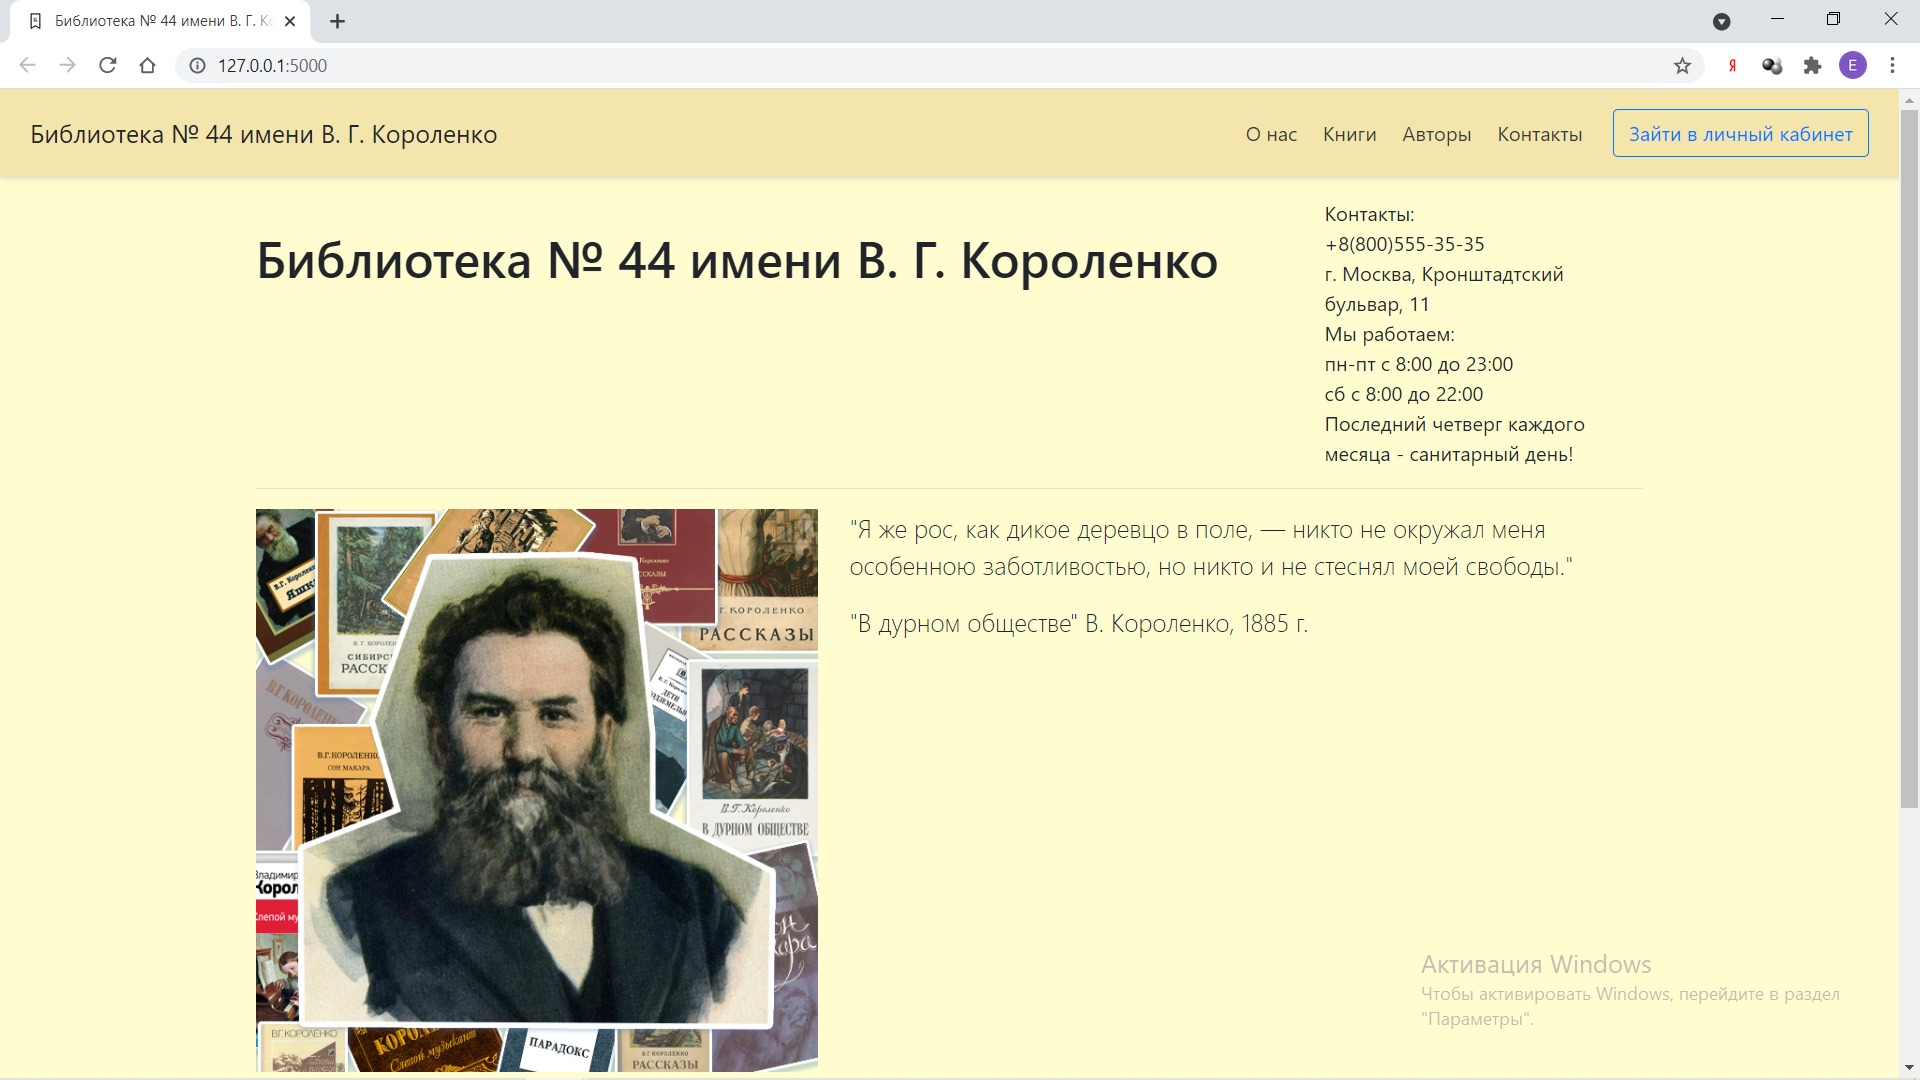
\includegraphics[scale=0.4]{img/Interface1.png}
	\caption{Стартовая страница.}
\end{figure}

\begin{figure}[h!]
	\centering
	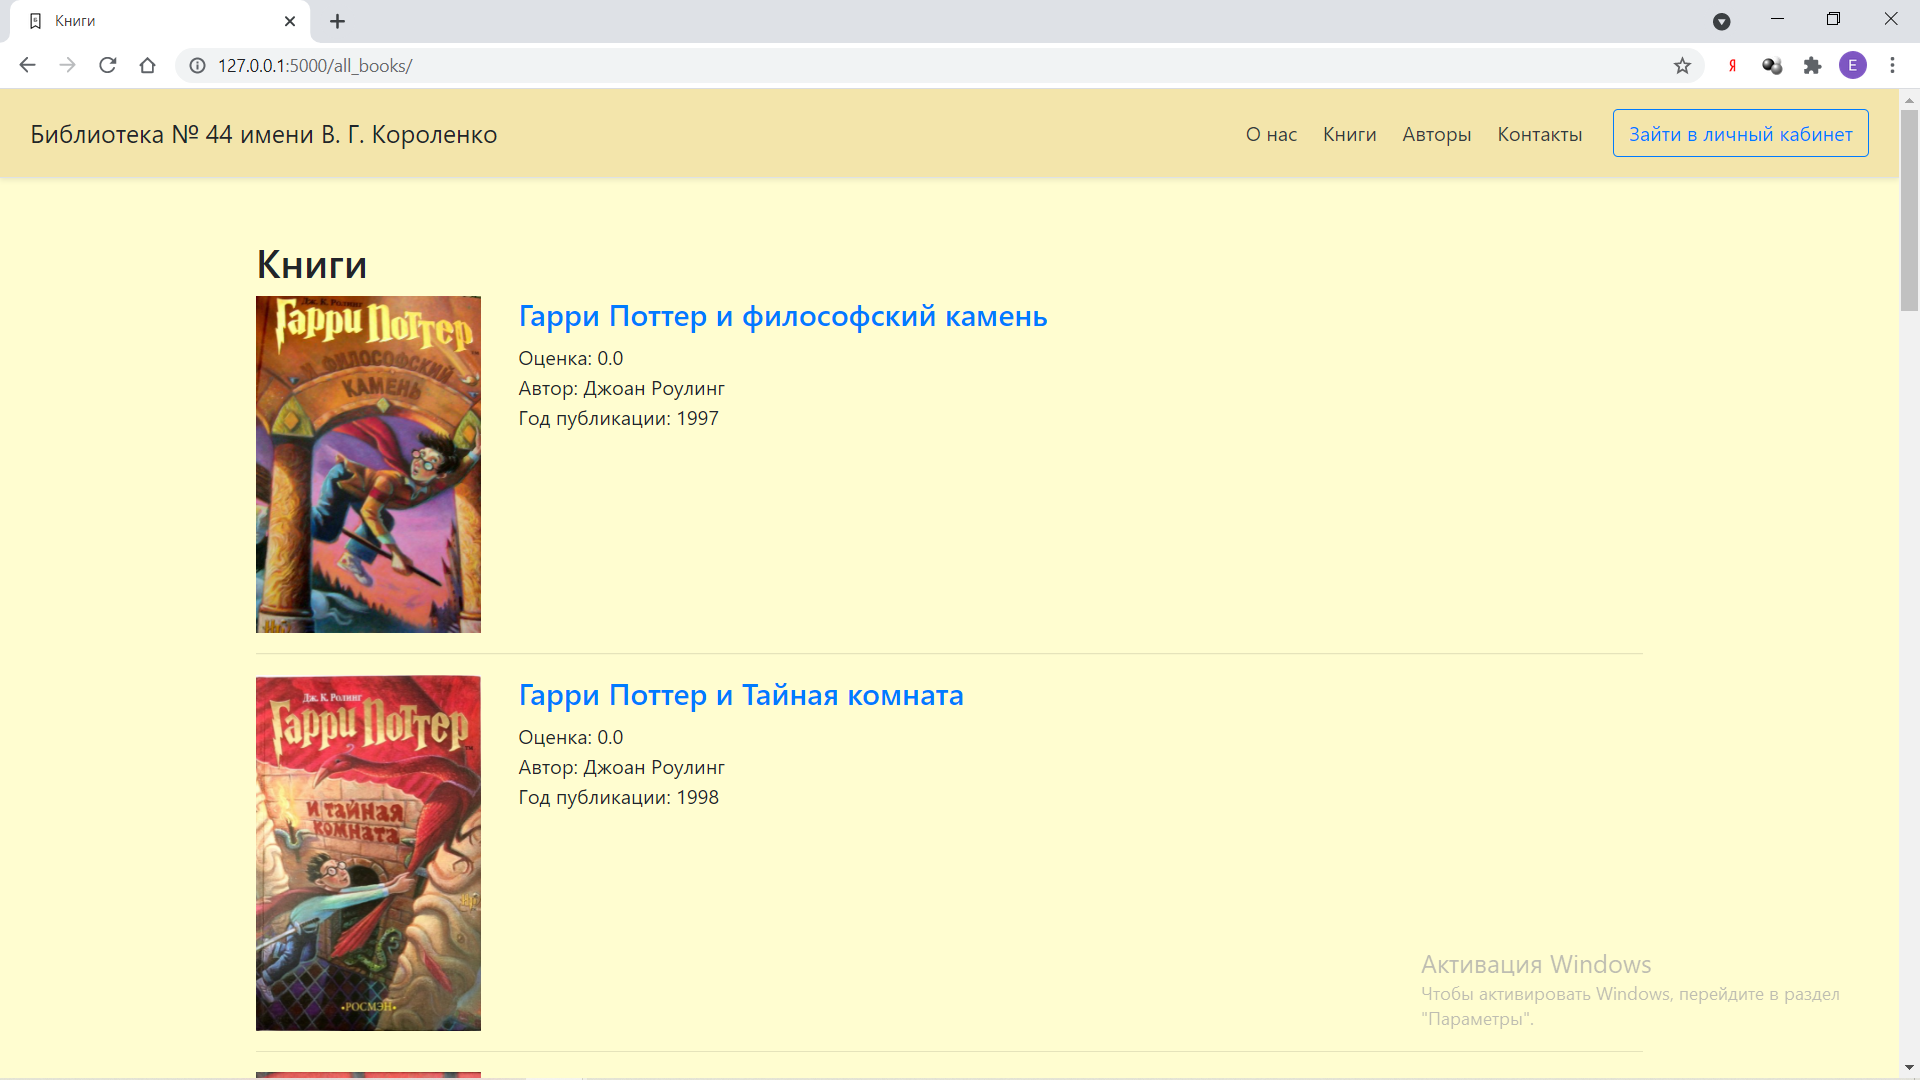
\includegraphics[scale=0.4]{img/Interface2.png}
	\caption{Список книг.}
\end{figure}

\begin{figure}[h!]
	\centering
	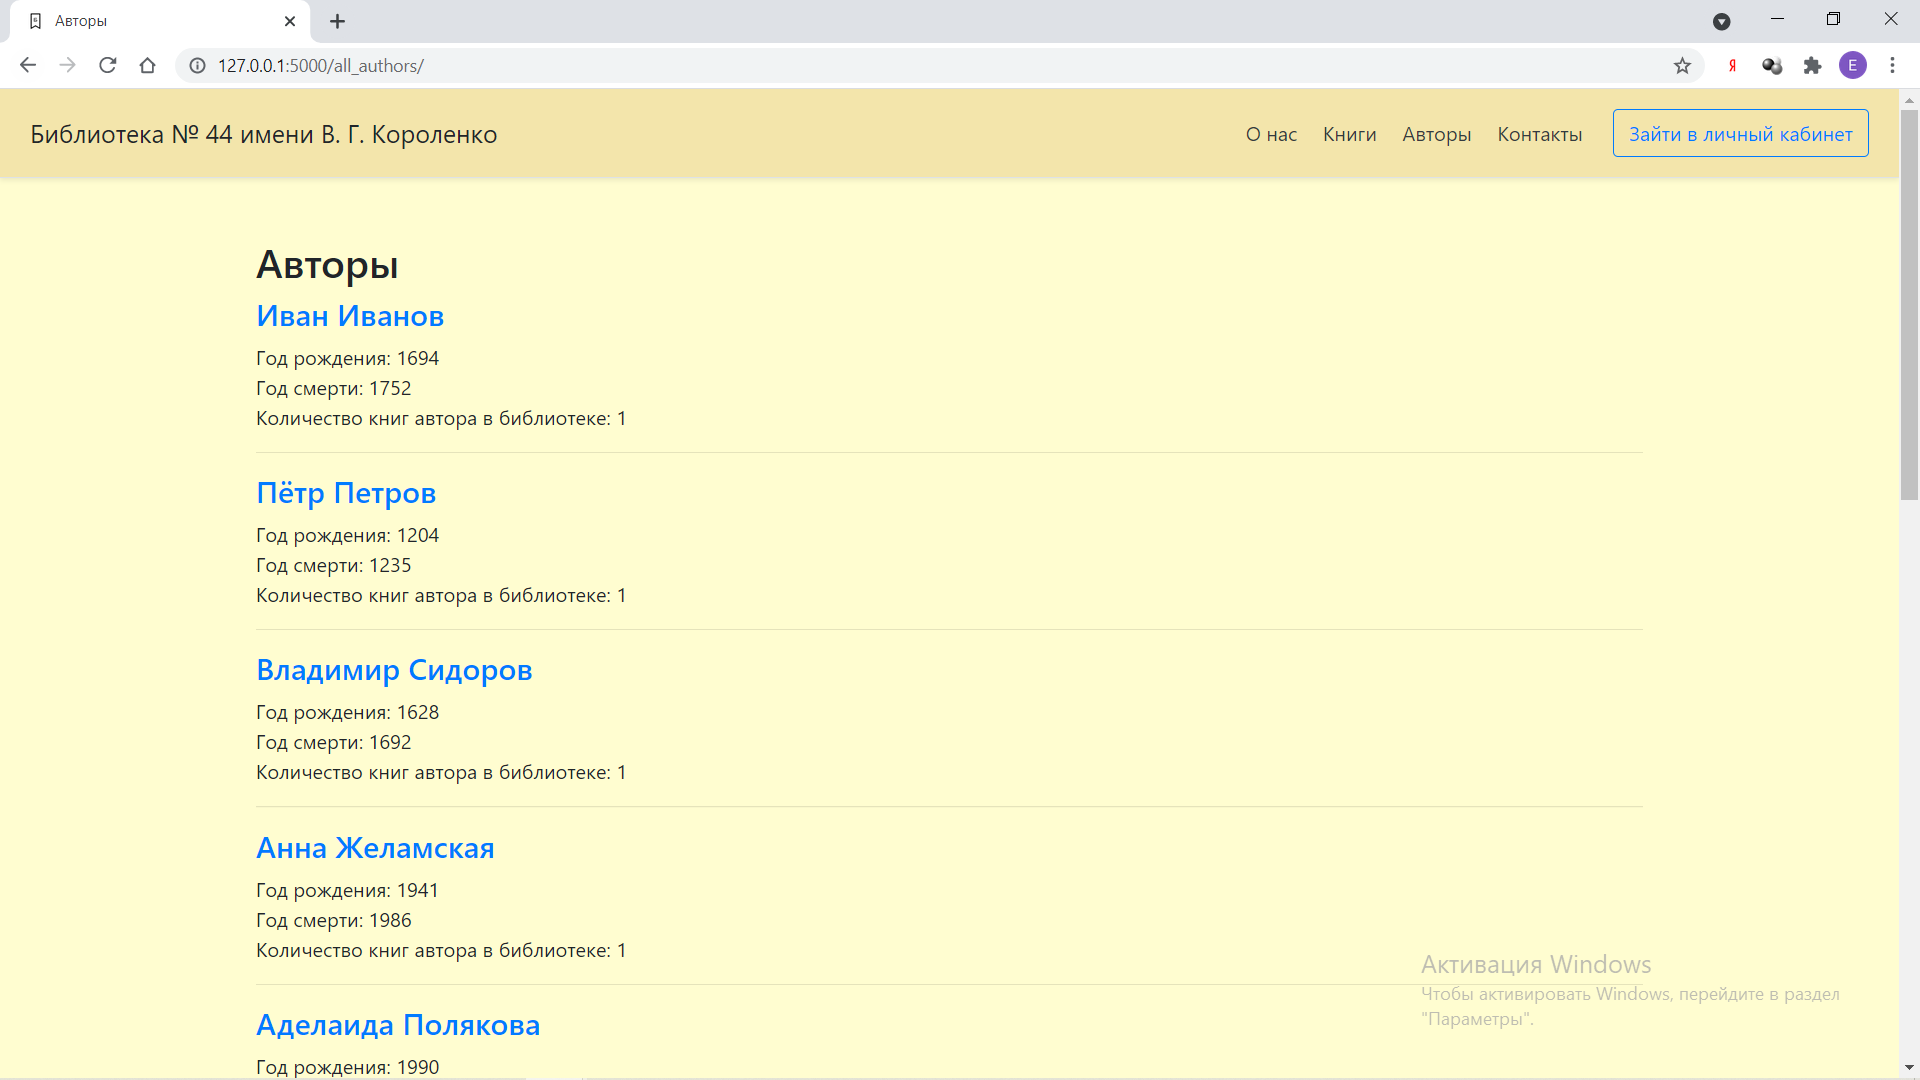
\includegraphics[scale=0.4]{img/Interface3.png}
	\caption{Список авторов.}
\end{figure}

\begin{figure}[h!]
	\centering
	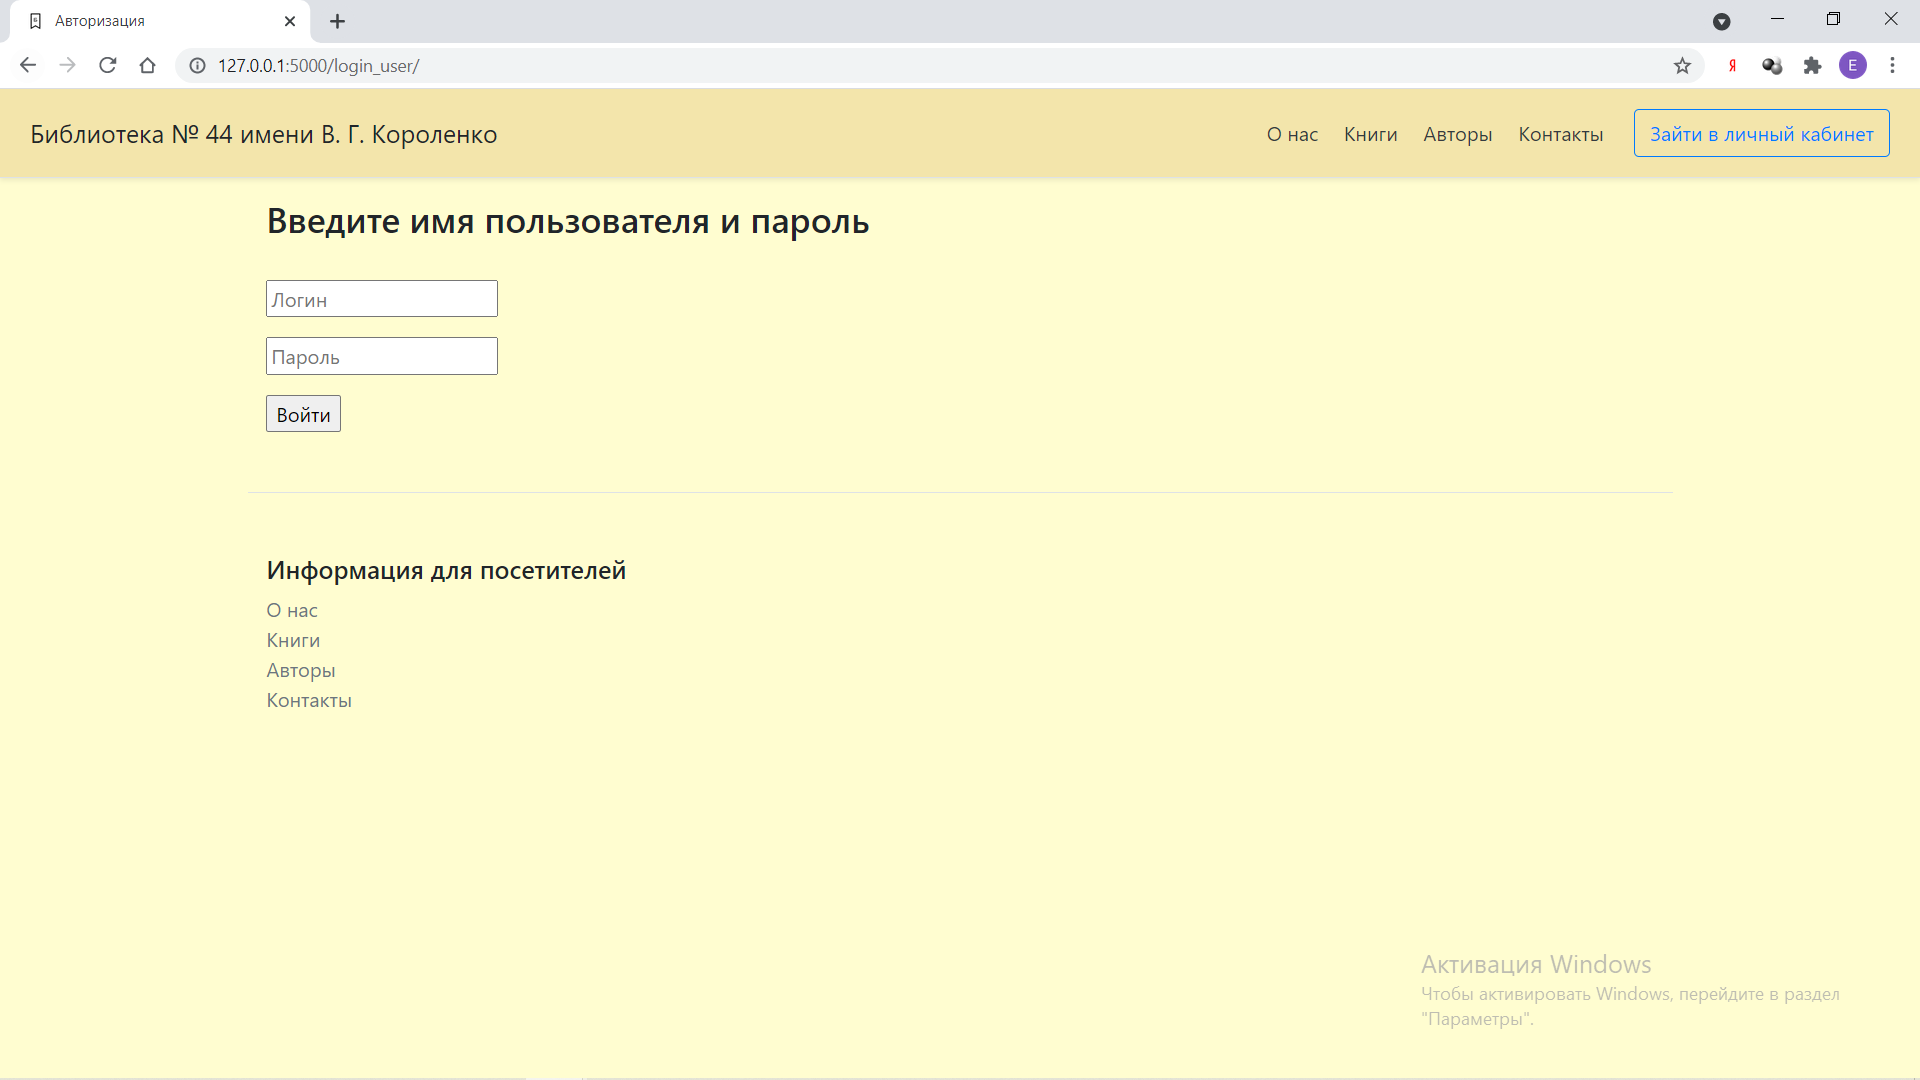
\includegraphics[scale=0.4]{img/Interface4.png}
	\caption{Авторизация.}
\end{figure}

\begin{figure}[h!]
	\centering
	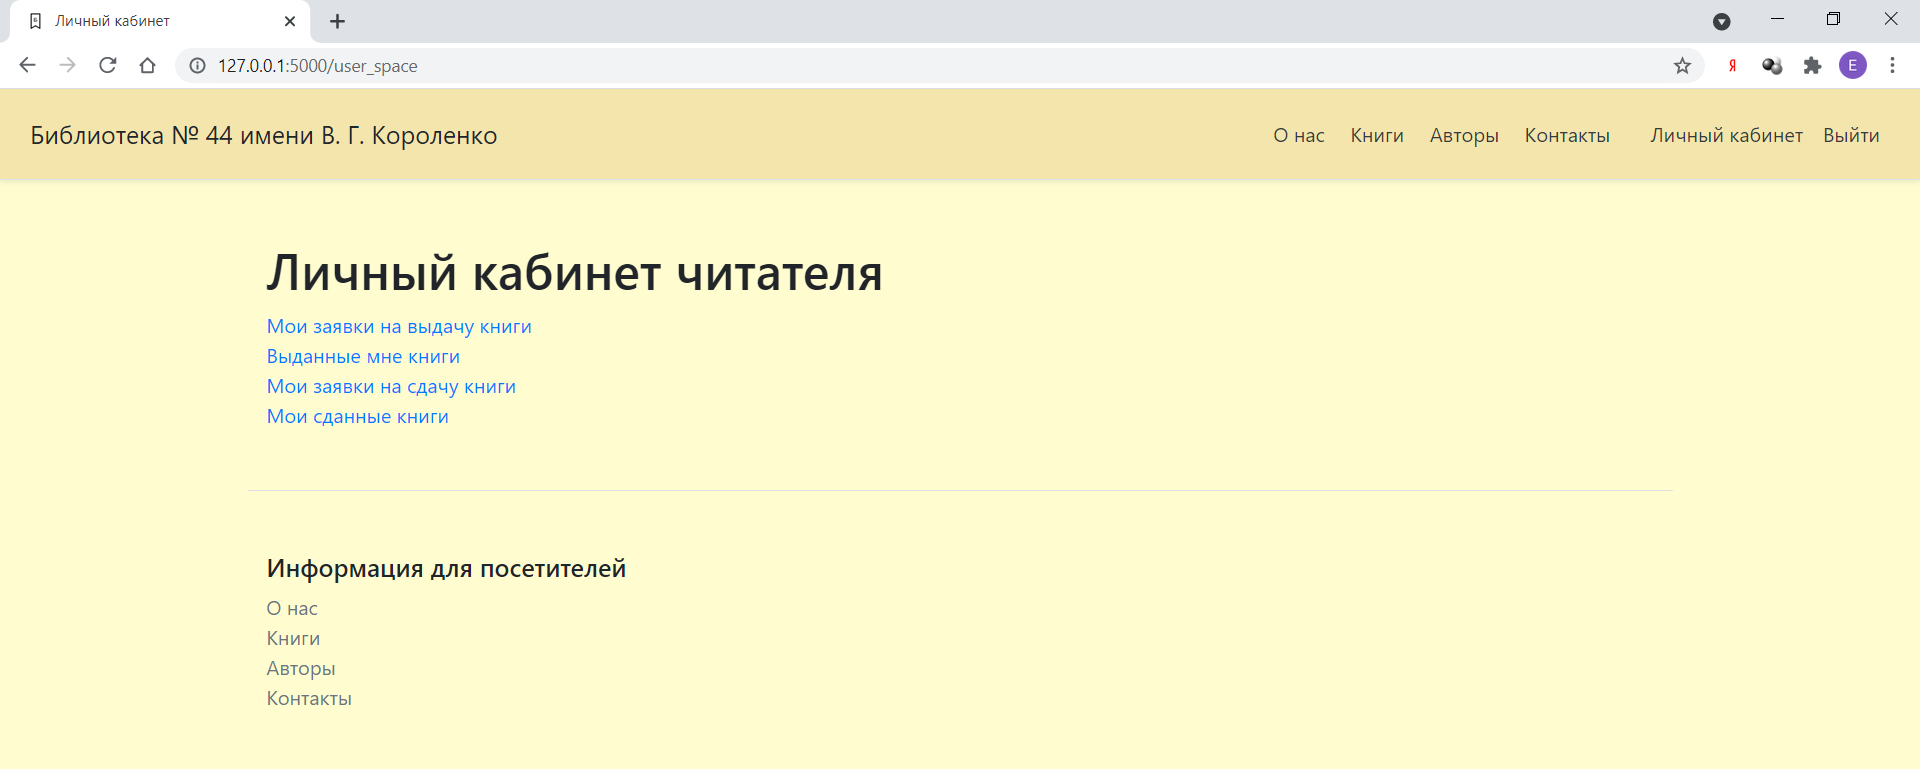
\includegraphics[scale=0.4]{img/Interface5.png}
	\caption{Личный кабинет читателя.}
\end{figure}

\begin{figure}[h!]
	\centering
	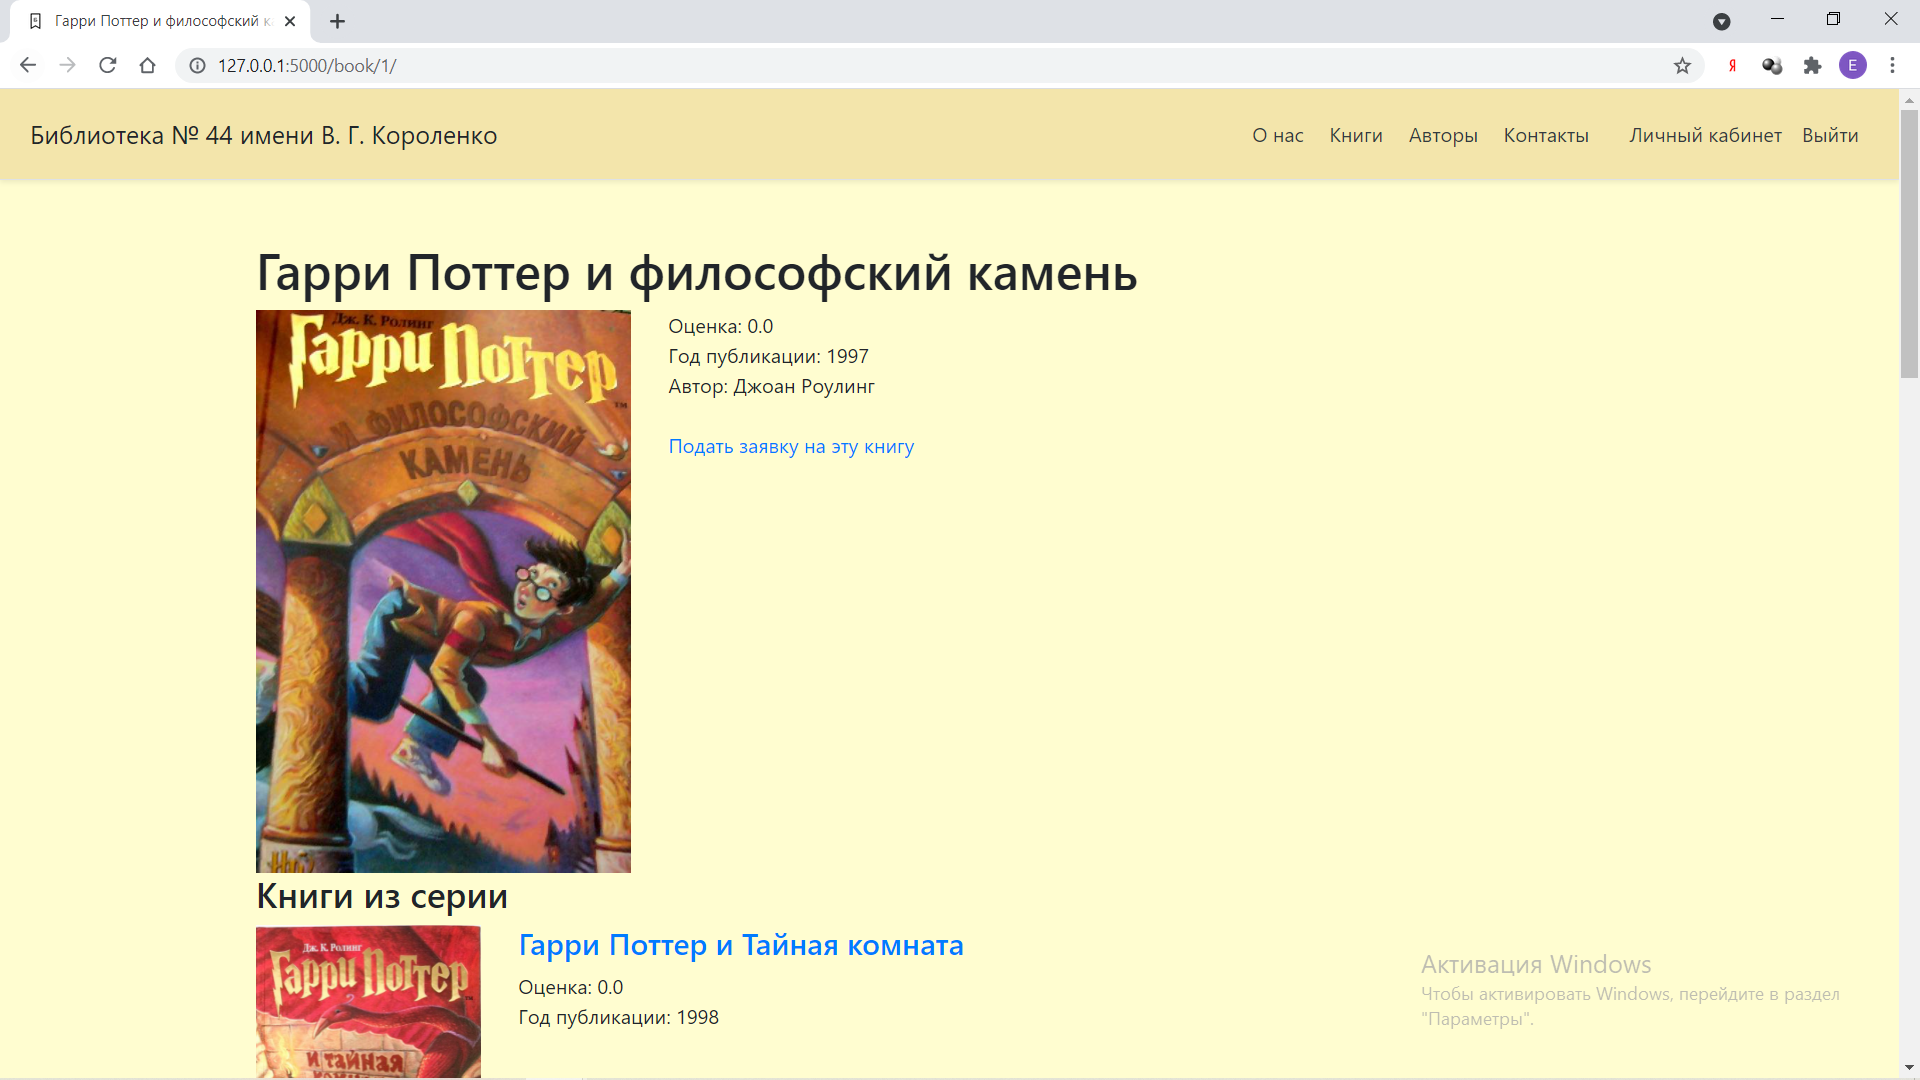
\includegraphics[scale=0.4]{img/Interface6.png}
	\caption{Страница книги.}
\end{figure}

\begin{figure}[h!]
	\centering
	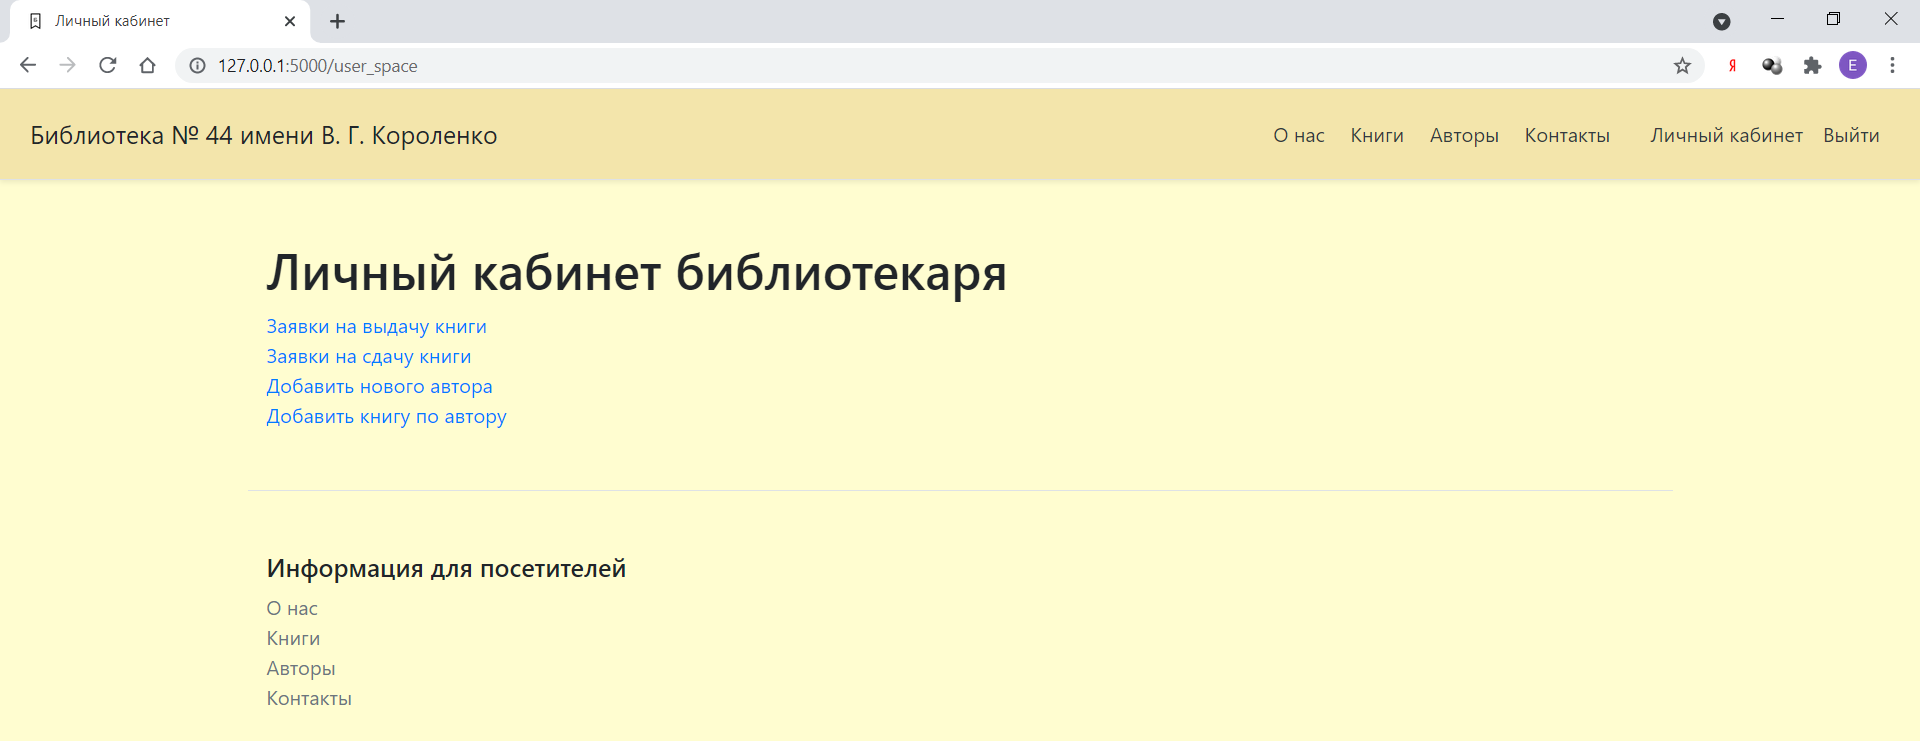
\includegraphics[scale=0.4]{img/Interface7.png}
	\caption{Личный кабинет библиотекаря.}
\end{figure}

\begin{figure}[h!]
	\centering
	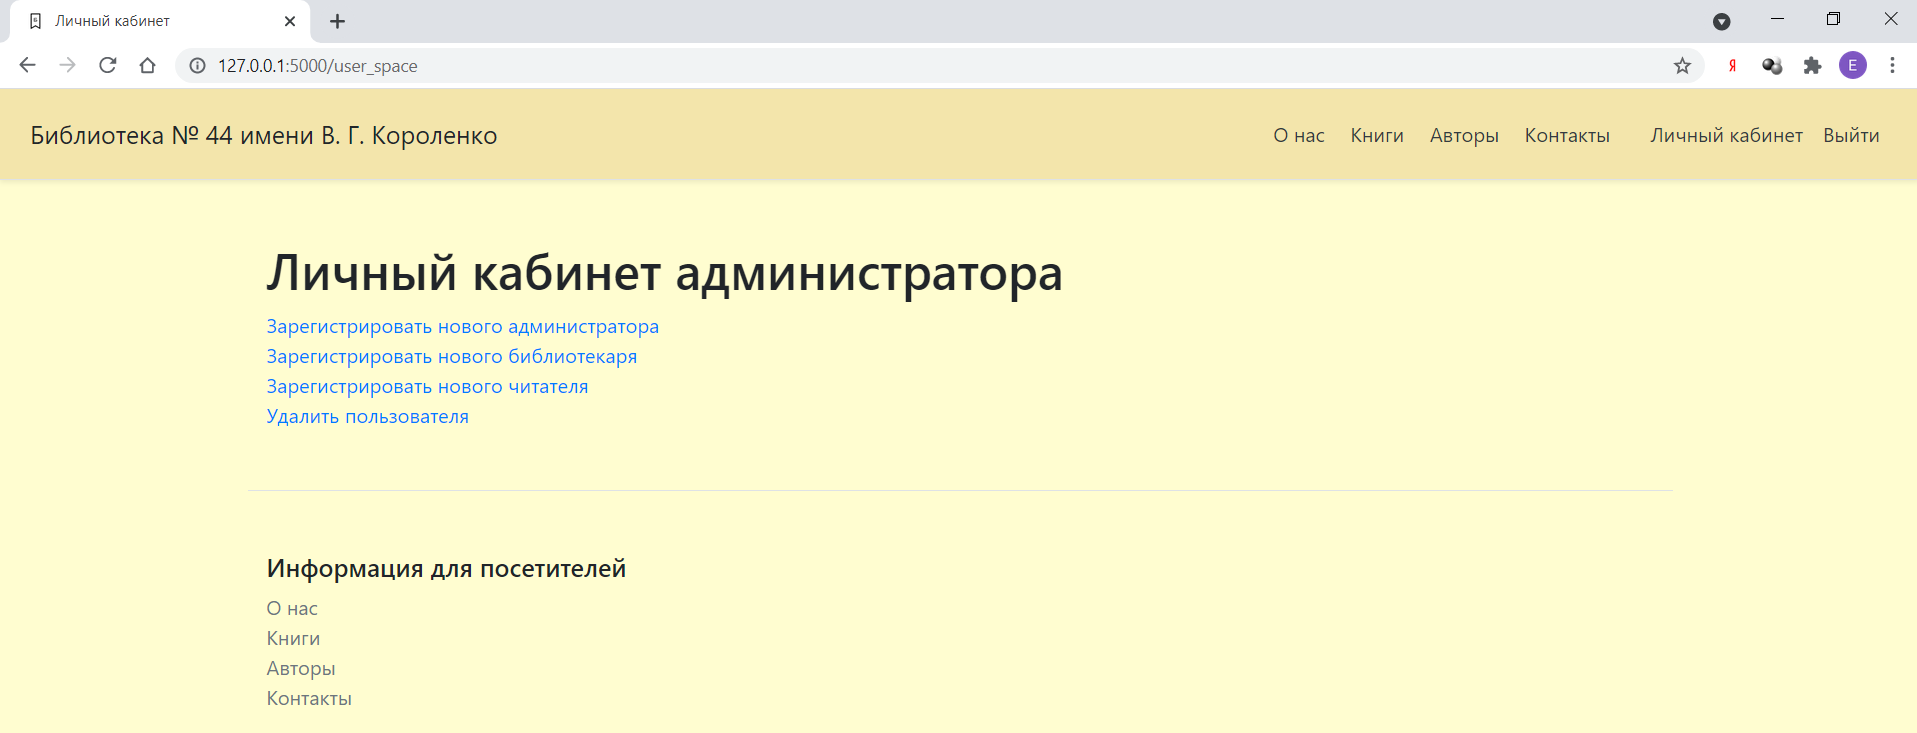
\includegraphics[scale=0.4]{img/Interface8.png}
	\caption{Личный кабинет администратора.}
\end{figure}
\clearpage

\subsection{Вывод}
В данном разделе были выбраны средства реализации поставленной задачи, создана база данных и описана ролевая модель на уровне БД, разработан о приложение.
\newpage
\section*{Заключение}
\addcontentsline{toc}{section}{Заключение}
Цель курсовой работы достигнута: разработаны база данных и приложение для библиотеки. Все задачи решены:
\begin{itemize}
	\item[1)] задание формализовано, акторы и их функционал выделены;
	\item[2)] проведен анализ СУБД и выбрана наиболее подходящая;
	\item[3)] спроектирована база данных;
	\item[4)] спроектирована архитектура приложения;
	\item[5)] разработано приложение.
\end{itemize}

Был получен опыт разработки базы данных.

\clearpage
%СПИСОК ЛИТЕРАТУРЫ
\begin{thebibliography}{9}
	\addcontentsline{toc}{section}{Литература}
	\bibitem{psql} PostgreSQL : Документация [Электронный ресурс] URL: https://postgrespro.ru/docs/postgresql (дата обращения: 20.09.2021);
	\bibitem{} Flask : Документация [Электронный ресурс] URL: https://flask.palletsprojects.com/en/1.1.x/ (дата обращения: 20.09.2021);
	\bibitem{} Python : Документация [Электронный ресурс] URL: https://www.python.org/doc/ (дата обращения: 20.09.2021);
	\bibitem{} Bootstrap : Документация [Электронный ресурс] URL: https://getbootstrap.com/ (дата обращения: 20.09.2021);
\end{thebibliography}

\addcontentsline{toc}{section}{Приложение А. Презентация.}

\end{document}